% !TeX root = paper.tex
\documentclass[a4paper,12pt]{article}

% Packages
\usepackage[utf8]{inputenc}     % For UTF-8 encoding
\usepackage{amsmath, amssymb}   % For math symbols
\usepackage{graphicx}           % For including graphics
\usepackage{geometry}           % For setting page margins
\usepackage{natbib}             % For citations
\usepackage{hyperref}           % For clickable links in references
\usepackage{subcaption}         % For side by side subfigures

% Page layout
\geometry{margin=1in}           % Set margins to 1 inch

% Title section
\title{Tina Paper In Development}
\author{Your Name}
\date{\today}

\begin{document}

\maketitle

\begin{abstract}
    This is the abstract of your paper. Briefly describe the purpose of the research, the main results, and the conclusions.
\end{abstract}

\section{Introduction}
The study of tree rings has proven useful across multiple fields, proving to be a reliable subject for reconstructing past climates of regional and local environments, as well as a mechanism to understand tree growth response \citep{fritts_dendroclimatology_1971} \citep{williams_using_2010} \citep{guibal_dendrochronology_2021} \citep{sheppard_dendroclimatology_2010}.
To obtain these data from the tree rings, it is necessary to measure tree rings from a tree cookie or core. The first high precision tool for this purpose was a stage micrometer, involving a trained technician to incrementally shift a tree core under the objective of a microscope - informing a computer when a new ring is encountered \citep{robinson_microcomputer_nodate}.
While this method has very high precision, the data is only as accurate as the experience and knowledge of the technician at the time of recording \citep{levanic_atrics_2007}.
The desire to remove repetition of errors in sampling and sampling bias across to individual technicians led researchers to an alternative - image analysis. 
\par
The first step in measuring tree ring width from images requires the digitization of the sample. There are currently two competing models to digitize a sample. The first model is to use a flatbed scanner or similar tool, providing the benefit to 

The first approach involved flatbed scanning technology which digitized the surface of a prepared sample \citep{guay_new_1992}. 
Flatbed scanners eventually encountered a resolution insufficiency when analyzing very narrow tree rings on the scale of a few cells. A new method introduced with the ATRICS system increased the resolution of samples by stitching together multiple images from a digital microscope camera \citep{levanic_atrics_2007}. 
ATRICS set an example of the process which has been implemented in two other image acquisition tools, Gigapixel and CaptuRING \citep{griffin_gigapixel_2021, garcia-hidalgo_capturing_2022}.
Both of these tools use professional cameras to take individual images of cores, although CaptuRING requires the technician to transfer the images to a second device and use the proprietary image stitching software PTGUI. 
A budget friendly image acquisition tool with integrated image stitching for both cores and cookies has yet to be released.   


% Potentially should have a section on tree ring width measurement software
% The images were then fed to software such as WinDENDRO to have technicians click tree rings on a graphical user interface (GUI) \citep{guay_new_1992}.
% More modern implementations of measurement software now exists which includes width measurement, cross dating, and autodetection of rings as well \citep{maxwell_measuring_2021}. 


\section{Methods}
The functionality of this system allows for the major steps in tree cookie and core digitization to be automated. Capturing images and stitching them together is handled without the need for user intervention. 
To do this, the system traverses the surface area of the sample after being given its dimensions. After the capturing process, the images are stitched and are stored on the device along with metadata of relevant 
settings and sample parameters.

\subsection{Hardware Design}

\subsubsection{Mechanical Structure}
The cartesian robot was purchased from an open source parts supplier, OpenBuilds. They sell various sets of gantry robots, motor controllers, and power supplies
which can be conveniently purchased from one supplier. All metal components are cut and sized, and have very detailed assembly videos, an active community forum,
and customer support to fall back on. The OpenBuilds ACRO system circumvents the need for most power tools, machining, electrical connectors, and technical knowhow that would otherwise be necessary to build a robust robot.
All other parts were designed using SolidWorks and printed on an FDM 3D printer using ABS material. Mechanical assembly can be completed entirely with common hand tools and metric fasteners. 

\subsubsection{Computer}
The computer which runs the graphical user interface (GUI), gantry control, camera streaming, and image stitching is the NVIDIA Jetson Orin Nano Developer Kit (Orin Nano). Using a computer
which is compatible with CSI cameras such as the Raspberry Pi HQ Camera was essential to maintain cost effectiveness. The Orin Nano, like others in the Jetson line of products, has hardware
accelerators for common GPU tasks such as image streaming, which is vital to retain CPU power for GUI tasks and robot control. 

\subsubsection{Camera}
Unlike the Gigapixel or CaptuRING, the camera is a machine vision camera rather than a handheld professional camera. Choosing the Raspberry Pi HQ Camera provided many lens options, significant
forum support, and includes an Obsolescence Statement that the camera will be in production until January 2030. Combined with a 180mm C-mount microscope lens, the images can reach above 20,000 dots per inch (DPI).

\subsection{Software Design}
All software was written in Python VERSION and a variety of packages for the GUI, image stitching, and calculations (Should I include all the packages in writing?). Care was taken to segment the
software design into abstracted object oriented code. 

\subsubsection{Graphical User Interface}
The GUI to control the machine launches from a Python script. Included are a viewer to see the live stream from the camera, buttons to jog the machine throughout the XYZ coordinate system,
setting the size of samples, and running the process to capture and stitch images. The system was designed to allow for multiple samples to be prepared in a queue for bulk digitization. 

\subsubsection{Sample Digitization}
The digitization of a sample can be reduced to a few processes - capturing a grid of overlapping images, image focusing, and image stitching. 

Inside the GUI, the program is populated with the height and width of the sample as well as the height and width of the image. The user then navigates to the center of the sample and can choose 
to begin imaging the sample or add the sample to a queue for bulk digitization. This provides the machine enough data to calculate the necessary rows and columns for traversing the entire surface
area of the sample while maintaining a level of overlap between adjacent images. Image overlap is what allows for images to be stitched together as there is nonzero error when the robot translates 
from one coordinate to another. 

To stitch adjacent images, feature based image stitching from a Python package Stitch2D was used. The underlying functions were based on the processing libraries
OpenCV and NumPy. Multiple other image stitching packages were tested but none were able to successfully piece together our samples. (***Sounds kinda bad to not have data on a comparison as well as not having a metric to see how 'well' an image is stitched... but this is non trivial. Can we get away with it?***)

One major difficulty with using the Raspberry Pi HQ Camera is the lack of a lens with auto-focus. An in focus image in this regime is dependent on the focal length of the lens set by the user and the
distance from the sample. The microscope lens has a very small depth of field and goes from in-focus to out-of-focus in less than a 1mm step in the distance to the sample. Two cooperative solutions were implemented 
to achieve a focused image for the entire surface area of the sample - taking images from multiple distances from the sample and automatic control. 

\subsubsection{Image Stack Focusing}
When the sample is placed on the table to be digitized, it is assumed that there will, at best, very slight variations in height across the surface area of the sample. A levelling table 
assists in reducing this error although it will never be nonzero. At each location (X, Y) on the grid of overlapping images, 11 images are captured in equally distanced Z steps across a 1mm range. 
Each of these images have a normalized variance score calculated - the maximum value represents the most in focus image \citep{sampat_extensive_2014}. In practice, stopping and starting the motor causes 
enough vibration to require upwards to two seconds of pause time before the motion blur stops to take each photo. Instead of stopping and starting each image, an additional distance is added to the 
Z-motion to allow the stepper to accelerate and reach constant velocity. At this speed, images are then taken with constant time steps instead of constant distance steps across the 1mm range. This eliminates
the motion blur due to acceleration and dramatically reduces imaging time. 

$$\frac{1}{MN\mu} \sum\limits_{x=0}^{M-1} \sum\limits_{y=0}^{N-1}(f(x,y) - \mu)^2$$

\subsubsection{Automatic Control}
While the image stack provides a basis to obtain an in focus image, it is statically limited to the 1mm range in the Z axis. Instead of spending significant time guaranteeing that the sample
is within the the Z axis range across the entire surface area, a PID control algorithm takes the wheel \citep{odwyer_summary_2000}. The information previously calculated in the image stack is sufficient 
to inform the PID controller of how to adjust the initial the Z axis for the next image stack. The controller is constantly trying to make the most in focus image be at the center of the image stack,
index value 5. This allows for the most flexibility moving to the next location of the image grid. 

\begin{figure}
    \centering
    \begin{subfigure}{.5\textwidth}
      \centering
      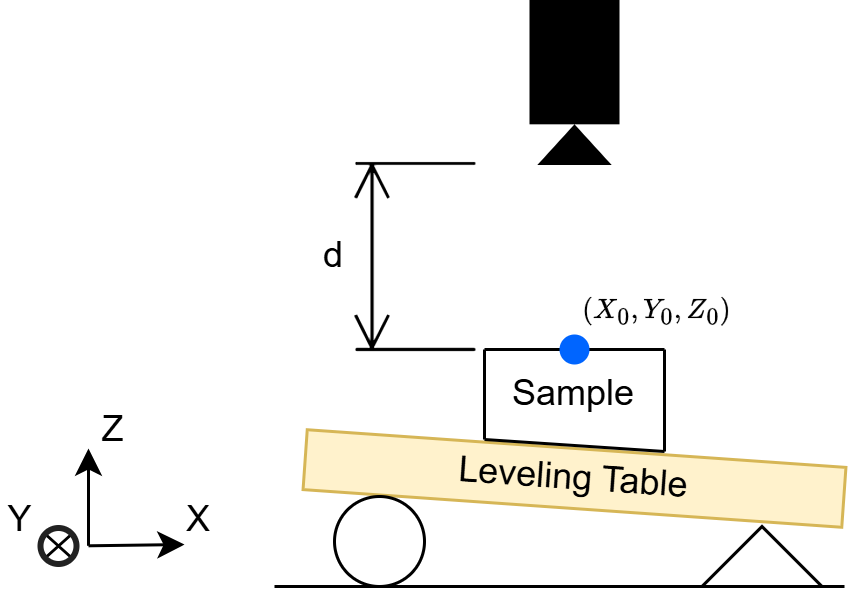
\includegraphics[height=0.75\linewidth]{../diagrams/sample_setup_ideal.png}
      \caption{Ideal sample leveling}
      \label{fig:sub1}
    \end{subfigure}%
    \begin{subfigure}{.5\textwidth}
      \centering
      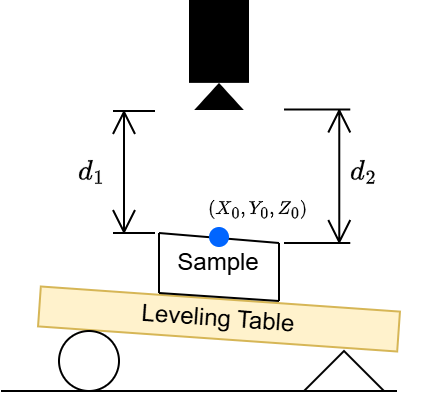
\includegraphics[height=0.75\linewidth]{../diagrams/sample_setup_realistic.png}
      \caption{Realistic sample leveling}
      \label{fig:sub2}
    \end{subfigure}
    \caption{Side view of the camera and sample on top of a leveling table. The ideal sample leveling shows a uniform distance d at all (x,y) coordinates on the sample. This is impossible to achieve in reality, the true sample leveling has a non uniform distance at unique (x,y) coordinates.}
    \label{fig:test}
\end{figure}


\section{Results}
\subsection{Scans of Cookies and Cores}
The microscope lens greatly improved the maximum resolution of the digitization. Resolutions of up to 13,400 DPI were achieved, a large improvement when compared to 
both high resolution flatbed scanners (Epson® Perfection v750 PRO) and CaptuRING. 

\subsection{Functional Limits}
With such high resolution, multiple logistics concerns arise. First is the file size. With such a high resolution, the size of the images can become extremely large. A cookie
5 inches in diameter would result in an image with 67,000 pixels squared. This easily exceeds the 2.5 GB maximum file size in a TIFF - most software for viewing the file will also 
be incompatible with any file this big as well. 


\section{Discussion}
Discuss the implications of your results here.

\subsection{Strengths and Opportunities}

\subsection{Opportunities for Improvement}

\section{Conclusion}
Summarize your key findings here.

\bibliographystyle{plainnat}
\bibliography{references}

\end{document}
